% Chapter Template

\chapter{Arbitrage Theory In Continuous Time Finance} % Main chapter title

\label{Chapter2} % Change X to a consecutive number; for referencing this chapter elsewhere, use \ref{ChapterX}

Arbitrage theory in continuous time finance is a very broad field with a lot of technical details. The focus on this chapter will to provide the basic tools and intuition for the arbitrage theory and lay the foundations for the computational finance methods. We follow the style in \parencite{Hull} and \parencite{finKont} to focus on intuition without going into the whelm of technicalities and proofs. We start with introducing the financial markets and key concepts for building arbitrage free and complete market models (see section \ref{FinMarket}). Then we actually build a framework for finding "fair" prices, i.e. finding a complete model with absense of arbitrage (see section \ref{MultiDimModel}). Lastly we go into specific cases where either numerical methods is needed or we have a closed-form solution (see section \ref{AmericanOptions} and \ref{classicBS}).

%----------------------------------------------------------------------------------------
%	SECTION 1
%----------------------------------------------------------------------------------------

\section{Financial Markets}\label{FinMarket}

\begin{figure}[th]
\centering
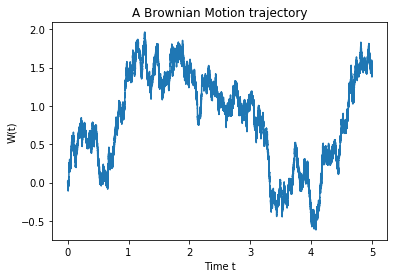
\includegraphics{Figures/brownianMotion.png}
\decoRule
\caption[A Wiener process trajectory]{}
\label{fig:BM}
\end{figure}


In the financial markets there is a lot of players and different types of investments. The classical investments are bonds and stocks, where you either lending or buying equity. The big players in the markets are commercial banks, investment banks, insurance companies and pension funds. Besides the classical investments types derivatives gives additional options for investments. A derivative are a financial instrument depending on an underlying asset, where the dependency is specified in the contract. The options in this thesis will all be stock options, but the techniques developed can easisy be extended to other types of derivatives. The contract of stock options can be constructed in many ways, where we in appendix \ref{AppendixA} included the put and call option. When pricing financial product we use the market to price derivatives (This correspond to the equivalent martingale measure $\mathbb{Q}$ to the objective measure $\mathbb{P}$), so we do not introduce arbitrage to the market. We will make idealized assumptions about the market:
\theoremstyle{assumption}
\begin{assumption}{}\label{EfficientMarket}
We assume following institutional facts:
\begin{enumerate}
\item[•] Short positions and fractional holding are allowed 
\item[•] There are no bid-ask spread, i.e. selling price is equal to buying price
\item[•] There are no transactions costs of trading.
\item[•] The market is completely liquid, i.e. it is possible to buy/sell unlimited quantities on the market. You can borrow unlimited amount from the bank by selling short.
\end{enumerate}
(see p. 6 \parencite{finKont})
\end{assumption}
We can discuss these assumptions at length, but in order to progress mathematically, we need to accept them for now. There is some justification for liquidity on vanilla options, because those options gets traded on large scale. Before going into the mathematics, we need to introduce some key concepts.
%-----------------------------------
%	SUBSECTION 1
%-----------------------------------

\subsection{Financial Derivatives}
There is a broad range of different derivatives. In this thesis, we will mainly divide derivatives into two classes. 
\begin{enumerate}
\item Simple derivatives (T-claims)
\item Exotic derivatives (e.g. American options)
\end{enumerate}
The first class is the simple derivatives. These are simple because you can only exercise them at maturity (time T). The exotic derivatives are all kind of functions on the underlying assets, where you can e.g. have an option to exercise from inception to maturity (see section \ref{AmericanOptions}) or a contract on several underlying stocks (see section \ref{BMHigherDim}). There are so many derivatives, hence the list will not be comprehensive at all. Some important simple derivatives will be the European calls and puts, because we can price analytically.

\theoremstyle{definition}
\begin{definition}{European Call Option:}\label{ECall}
A European call option is an option where the owner of the option has the option to exercise at maturity. The contract function for the derivative:
\begin{equation}
\begin{split}
\Phi(S(T))=\max\{S(T)-K, 0\}
\end{split}
\end{equation}
Where S(T) is the price of underlying asset at maturity and K is the agreed strike price.
\end{definition}
For illustration of above contract see appendix \ref{AppendixA} \parencite{finKont}.


%-----------------------------------
%	SUBSECTION 2
%-----------------------------------

\subsection{Self-financing Portfolio (Without Consumption)}
A self-financing portfolio h, is a portfolio h which doesn't get any external injection of money. h is the number of each assets in our portfolio. We denote $V^{h}(t)$ the value of our portfolio h at time t, hence:
\theoremstyle{definition}
\begin{definition}{Self-financing portfolio}
A portfolio consisting of n+1 assets: \\
h(t)=($h_0(t),h_1(t), \dotsc, h_{n}$) is self-financing if:
\begin{equation}\label{SF}
\begin{split}
dV^{h}(t)=\sum_{i=0}^{n} h_{i}(t) dS_{i}(t)
\end{split}
\end{equation}
Where $S_{i}$ is the $i'th$ asset in our portfolio, n+1 is the total number of assets and\\
$V^{h}(t)=\sum_{i=0}^{n} h_{i}(t) S_{i}(t)$
\end{definition}
The important takeaway is that a S-F portfolio is kind of a budget restriction. You are only allowed to reallocate your assets within the portfolio but not injecting cash into the portfolio. The concept is important for the discussion of arbitrage and hedging \parencite{finKont}.

%-----------------------------------
%	SUBSECTION 3
%-----------------------------------
\subsection{Arbitrage}
Arbitrage is the financial term for a "free lunch". If there is arbitrage in the market an investor can profit without bearing risk. In order to avoid making a "money machine", we want to price derivatives by not introducing arbitrage to the market.  
\theoremstyle{definition}
\begin{definition}{Arbitrage:}
An arbitrage possibility on a financial market is a self-financed portfolio h suct that
\begin{equation}\label{Arbitrage}
\begin{split}
V^{h}(0)=0\\
P(V^{h}(T)\geq 0)=1\\
P(V^{h}(T)>0)>1
\end{split}
\end{equation}
We say that the market is arbitrage free if there aro no arbitrage possibilities.\\
(see p. 96 \parencite{finKont})
\end{definition}
From the definition of a self-financing portfolio fulfilling equation \eqref{Arbitrage} would give the possibility for arbitrage. The investor in this portfolio starts with 0 dollars, and without injecting any money, the investor is certain of not losing any money. In addition he has a positive probability by ending up with more than 0 at maturity. Arbitrage is a way to price financial products "fair". To price "fair" and hedge against risk will be the topics for the rest of this thesis.

%-----------------------------------
%	SUBSECTION 4
%-----------------------------------

\subsection{Complete Market And Hedging}
Hedging is a concept to protect against exposure to risk. A hedge is simply a risk neutralization action in order to minimize the overall risk. In the definition below, we define a hedge for an simply T-claim.
\theoremstyle{definition}
\begin{definition}{Hedging and completeness for T-claim:}
A T-claim X can be hedged, if there exist a self-financing portfolio h such that:
\begin{enumerate}
\item[•] $V^{h}(T)=X$ P-a.s.
\end{enumerate}
I.e. h is an hedge portfolio for X if it is guaranteed to pay in all circumstances an amount identical to the payout of X.\\
The market is complete, if every derivative is hedgeable.
(see p. 192fa \parencite{finKont})
\end{definition}
Hedging and completeness means the same for other derivatives than T-claims, but for now we will only show the concepts for the T-claim. By defining the fundamental concepts we are ready to solve the two fundamental problems:
\begin{enumerate}
\item[•] Pricing derivatives without introducing arbitrage to the market.
\item[•] When is the market complete?
\end{enumerate}

%----------------------------------------------------------------------------------------
%	SECTION 2
%----------------------------------------------------------------------------------------

\section{Multidimensional Models}\label{MultiDimModel}
There is two main method for deriving arbitrage free and complete markets. The classical approach is the delta hedging approach \parencite{B-S-Paper} and \parencite{CRR}). The more advanced mathematical approach is the martingale approach  \parencite{finKont}. In this section we will focus on the martingale approach and show the delta hedging approach is a special case of the more general martingale theory. For the martingale approach the First and Second Fundamental Theorems of Mathematical Finance will be the key for obtaining a fair market. Besides the model assumptions will we also assumes the financial market assumptions in section \ref{FinMarket}.

\subsection{Model Assumptions}
Let us consider a filtered probability space $(\Omega, \mathcal{F}, P, \mathcal{F}_t^{\bar{W}})$. Note the assumption that filtration is only generated from the Wiener process, so the $\bar{W}$ is the only random source and we assume $\bar{W}_i$ is k-dimensional. I.e. we assume that we are in a Wiener world, where all processes are Wiener driven. A priori we assume a market $(B(t),S_1(t), S_2(t),\ldots, S_n(t))$, where ${S_i(t)}_{i=1,2,\ldots,n}$ is n risky assets S(t) and B(t) is the risk free asset. By assumptions their dynamics are given by:\\
\begin{align}
dS(t)=D[S(t)]\alpha(t)dt+D[S(t)]\sigma(t)d\bar{W}(t)\label{GBM-P} \\
dB(t)=r(t)B(t)dt
\end{align}
We assume $\alpha_i$, $\sigma_{ij}$ and the short rate $r(t)$ are adapted processes.
For convenience we used vector and matrix notation for the GBM process.\\
n risky assets
$$S(t)=\begin{pmatrix}
S_1(t)\\
S_2(t)\\
\vdots\\
S_n(t)
\end{pmatrix}
$$
k dimensional Wiener processes:\\
$\bar{W}(t)=\begin{pmatrix}
\bar{W}_1(t)\\
\bar{W}_2(t)\\
\vdots\\
\bar{W}_n(t)
\end{pmatrix}
$\\
volatility matrix $\sigma=\{\sigma_{ij}(t)\}_{i=1,\ldots,n,j=1,\ldots,k}$, local mean of rate of return vector $\alpha=(\alpha_1(t), \alpha_2(t), \ldots, \alpha_n(t))^T$, and D(x) denotes a diagonal matrix with vector x as its diagonal.\\ 
Furthermore the Wiener processes covariance is $Cov(dW_i(t)dW_j(t))=\rho_{ij}dt$ where $\rho_{i,i}=1$

\subsection{Arbitrage Free Model}
The first problem we are faced with in arbitrage theory is to price the derivative, i.e. finding $\Pi(t,\mathcal{X})$ the price at time t without introducing arbitrage to the market $(B(t), S(t), \Pi(t))$. The First Fundamental Theorem tells us how to price $\Pi(t)$.
\begin{theorem}\label{FFT1}
\textbf{First Fundamental Pricing Theorem of Mathematical Finance(FFT1): } The market model is free of arbitrage if and only if there exist a martingale measure, i.e. a measure $Q\sim P$ s.t. the processes:
$$\frac{S_0(t)}{S_0(t)}, \frac{S_1(t)}{S_0(t)}, \cdots, \frac{S_n(t)}{S_0(t)}$$
are (local)martingales under Q.
(see p. 154 \parencite{finKont})
\end{theorem}

From the FFT1 with the bank account B(t) as numeraire, we have:
\theoremstyle{proposition}
\begin{proposition}{}
We assume that $B(t)=S_0(t)$ is our numeraire and all the processes are Weiner driven, then a equivalent measure $Q \sim P$ is martingale measure if and only if all assets $(B(t), S_1(t), \ldots, S_n(t))$ have the short rate as their local rates of return, i.e.
\begin{align}
dS_i(t)=S_i(t)r(t)dt+S_i(t)\sigma_i(t)dW^Q(t)
\end{align}
(see p. 154 \parencite{finKont})
\end{proposition}
So to not introduce arbitrage to the model for the market, we need to ensure the Q-dynamics of S is:
\begin{equation}\label{Q-dym}
dS(t)=D[S(t)]r(t)dt+D[S(t)]\sigma(t)d\bar{W}(t)
\end{equation}
The tool to obtain the dynamics in eq. (\ref{Q-dym}) is Girsanov Theorem (see \ref{Girsanov}). Girsanov Theorem is a continuous measure transformation, where in our model we want to transform the dynamics given with the objective probability measure P to an equivalent martingale measure Q (i.e. the martingale measure chosen by the market). By suitable chooses of the likelihood process L and setting $dQ=L(T)dP$, then with Girsanov theorem we can write:
$$d\bar{W}(t)=\phi(t)dt + dW(t)$$
When applying to eq. (\ref{GBM-P}):
$$dS(t)=D[S(t)](\alpha(t)+\sigma(t)\phi(t))dt+D[S(t)]\sigma(t)d\bar{W}(t)$$
Going back to the FFT1 and the proposition, we know that Q is martingale measure if and only if:
\begin{align}\label{marketPriceOfRisk}
\alpha(t)+\sigma(t)\phi(t)=\textbf{r}(t) \quad holds \ with \ probability \ 1 \ for \ each \ t
\end{align}
By above discussion and disregarding "pathological models" (will use the term generically arbitrage free when pathological models are not considered). Furthermore we assume enough integrability and we have the following useful result:
\theoremstyle{proposition}
\begin{proposition}{}\label{arbitrageFreeProp}
Disregarding integrability problems the model is generically arbitrage free if and only if, for each $t\leq T$ and P-a.s. the mapping:
$\sigma(t):\mathbb{R}^k \to \mathbb{R}^n$ is surjective, i.e. if and only if the volatility matrix $\sigma(t)$ has rank n.
(see p. 198 \parencite{finKont})
\end{proposition}
We note that in order not to have arbitrage in our model, we need $k\geq n$, i.e. have at least as many random sources as number of risky assets.

\subsection{Complete model}
Second Fundamental Pricing Theorem is key to obtain a complete market model, i.e. a market model where every claim can be hedged.
\begin{theorem}\label{FFT2}
\textbf{Second Fundamental Pricing Theorem of Mathematical Finance(FFT2): } Assuming absence of arbitrage, the market model is complete if and only if the martingale measure $Q$ is unique.
(see p. 155 \parencite{finKont})
\end{theorem}
Hence in our Wiener world we have a unique martingale measure if eq. \ref{marketPriceOfRisk} has a unique solution. 

\begin{proposition}{}\label{completeProp}
Assume that the model is generically arbitrage free and that the filtration is defined by:
$$\mathcal{F}_t=\mathcal{F}_t^{\bar{W}}$$
Then disregarding integrability problems, the model is complete if and only if k=n and the volatility matrix $\sigma(t)$ is invertible P-a.s. for each $t \leq T$
(see p. 200 \parencite{finKont})
\end{proposition}


\subsection{Pricing and connection to classical approach}
The pricing formula for arbitrage free market model is the risk neutral valuation formula:
\begin{proposition}{}\label{RNVF}
To avoid arbitrage, $\mathcal{X}$ must be priced according to the formula:
\begin{align}
\Pi(t;\mathcal{X})=S_0(t)E^Q[\frac{\mathcal{X}}{S_0}|\mathcal{F}_t]
\end{align}
Note if we choose our numeraire $S_0(t)=B(t)$ then
\begin{align}
\Pi(t;\mathcal{X})=E^Q[\exp(-\int_t^T r(s) ds) \mathcal{X}|\mathcal{F}_t]
\end{align}
(see p. 155 \parencite{finKont})
\end{proposition}

The classical approach to arbitrage free and complete market models is based on a Markovian model assumption and k=n. Assume we are in a Wiener world, where the probability space $(\Omega, \mathcal{F}, P, \mathcal{F}_t^{\bar{W}_t}$ is given. Furthermore we assume $\alpha$ and $\sigma$ are deterministic functions and constant over time. $\sigma$ is also assumed invertible. Under these more restrictive assumptions the risk neutral valuation formula for a simple T-claim is given by the Markov property:
\begin{align}\label{MarkovRNVF}
\exp(-r(T-t))E^Q[\mathcal{X}|S(t)]
\end{align}

Applying Kolmogorov backward equation on eg. \ref{MarkovRNVF}, we obtain the BS-PDE for the pricing function F(t,S(t))=$\Pi(t; \mathcal{X})$.

\begin{theorem}\label{BSPDEMultiDim}
\textbf{Black Scholes PDE: } Consider the contract $\mathcal{X}=\Phi(S(T))$. In order not to introduce arbitrage to the market, the pricing function $F(t,s)$ must solve the boundary value problem.(TODO)
\begin{equation}
\begin{split}
F_t(t,s)+rsF_s(t,s)+\frac{1}{2} s^2 \sigma^2(t,s)F_{ss}(t,s) -rF(t,s)&=0\\
F(T,s)&=\Phi(s)
\end{split}
\end{equation}
(see p. 155 \parencite{finKont})
\end{theorem}


%----------------------------------------------------------------------------------------
%	SECTION 3
%----------------------------------------------------------------------------------------
\section{Classical Black-Scholes Formulas}\label{classicBS}
We will not do the classical delta hedging approach in \parencite{B-S-Paper}. Instead we use the general multidimensional martingale approach to derive the essential formulas for pricing. 
To derive a closed-form solution to the European call and put option, we concentrate at a special case of the multidimensional framework, where we only have the risk free asset and one risky asset. 
We further restrict ourselves to:\\
\theoremstyle{assumption}
\begin{assumption}{Black-Scholes assumptions}\label{BS-Assumption}
We assume following ideal conditions in addition to \eqref{EfficientMarket}:
\begin{enumerate}
\item[•] The short-term interest rate is known and is constant through time 
\item[•] The stock price follows a Geometric Brownian Motion. The $\sigma$ is constant.\item[•] The stock pays no dividends or other distributions.
\item[•] The option is a simple option ("European" see \eqref{ECall}).
\end{enumerate}
(see p. 640 \parencite{B-S-Paper})
\end{assumption}

We assume the underlying stock follows a geometric brownian motion:
$dS(t)=\alpha S dt + \sigma S dW_t$ where the solution to the SDE is given as
\begin{equation}\label{GBM}
\begin{split}
S(t)=S(0) \cdot \exp \bigg( (\alpha -\frac{1}{2} \sigma^2) t + \sigma W(t) \bigg)
\end{split}
\end{equation}
Where $\alpha$ is the local mean rate of return and $\sigma$ is the volatility of S. By above assumptions we are in a Markovian model, and we know the Black Scholes PDE in this setup (see eq.  \ref{BSPDEMultiDim}). By Feynman-Kac we have the risk neutral valuation formula.

\begin{theorem}\label{BRNVF}
\textbf{Risk-neutral valuation formula:} Given Q is the martingale measure
\begin{align}
\Pi(t, X)= exp(-r(T-t))\cdot E_{t,x}^Q[X]
\end{align}
\end{theorem}
From the RNVF we can derive a closed form solution for both a European call and put option. We will provide the European call option and the put-call-parity, because from the put-call-parity relationship we derive the European put option from the call option.

\theoremstyle{proposition}
\begin{proposition}{}\label{BS-price-EuroCall}
\textbf{Black-Scholes formula for call option:} The price of a European call option with strike K and maturity T is given by the formula  $\Pi(t)=F(t,S(t)$, where
\begin{align*}
F(t,s)=s \cdot N(d_1(t,s)) - e^{-r(T-t)}\cdot K \cdot N(d_2(t,s))
\end{align*}
N is the cumulative distribution function of a standard normal distribution $\mathcal{N}(0,1)$ and
\begin{align*}
d_1(t,s)=\frac{1}{\sigma\cdot \sqrt{T-t}} \cdot \bigg( \ln(\frac{s}{K}) + (r+\frac{1}{2} \sigma^2) (T-t) \bigg)\\
d_2(t,s)=d_1(s,t)-\sigma \sqrt{T-t}
\end{align*}
(see p. 105 \parencite{finKont})
\end{proposition}

\theoremstyle{proposition}
\begin{proposition}{}\label{put-call-parity}
\textbf{Put-call parity:} 
Assume the call and put option has same strike price and time to maturity.
\begin{align*}
p(t,s)=K\cdot \exp(-r(T-t))+c(t,s)-s
\end{align*}
(see p. 126 \parencite{finKont})
\end{proposition}

The put-call-parity holds only for European options, but the framework developed in this section will be useful for benchmarks and control variate for the numerical procedures.

The above formula for the European call option is actually the same for an American call option, but is not true for an American put option or for call options paying dividends. The result for the American call option was shown by Merton \parencite{Merton73}, that the intrinsic value is never greater than the worth of the option given by the risk-neutral valuation formula. In section \ref{AmericanOptions} we will show a martingale approach to prove the value of a European and American call coincides when the underlying is a non-dividend paying stock \parencite{finKont}.

%----------------------------------------------------------------------------------------
%	SECTION 4
%----------------------------------------------------------------------------------------

\section{American Options And Optimal Stopping}\label{AmericanOptions}
The American options adds additional complexity to the pricing problem, because compared to the European option the American option can be exercised at any time from inception to maturity. The main problem with American options is to find a optimal stopping time, i.e.
\begin{align}
\max_{0 \leq \tau\leq T}\{E[\Phi(\tau,X_{\tau})]\}
\end{align}
Where $\tau$ is a stopping time (see definition \ref{stopTime}).
We assume satisfied integrability condition on a finite interval $[0,T]$:
$$\sup_{0 \leq \tau\leq T}\{E[\Phi(\tau,X_\tau)]\}<\infty$$
and assume a diffusion setting:
$$dX_t=\mu(t,X(t))dt + \sigma(t,X(t))dW(t)$$

To find the optimal stopping time we introduce the optimal value function V(t,X(t)).
\theoremstyle{definition}
\begin{definition}{Optimal value function }\label{optValFunc}
For fixed $(t,x)\in [0,T]X\mathbb{R}$, and each stopping time $\tau$ with $\tau\geq t$ the optimal value function $V(t,x)$ is defined by
\begin{align}
V(t,x)=\sup_{t \leq \tau\leq T}\{E[\Phi(\tau,X_{\tau})]\}
\end{align}
A stopping time which realizes supremum for V is called optimal and be denoted $\hat{\tau}_{tx}$.
(see page 341 \parencite{finKont})
\end{definition}
By using a dynamic programming argument with three strategies:
\begin{enumerate}
\item[•] Use optimal stopping strategy $\hat{\tau}_t$
\item[•] Stop immediately
\item[•] Wait one time-step h and then use optimal stopping strategy $\hat{\tau}_{t+h}$
\end{enumerate}
Jumping over some argument and like in this section assuming "enough regularity", we arrive at two important propositions for numerically evaluating American options.

\begin{proposition}{\textbf{variational inequalities}}\label{varInEq}
Given enough regularity, the optimal value function is characterized by the following relations:
\begin{equation}
\begin{split}
V(T,x)=\Phi(T,x)\\
V(t,x)\geq \Phi(t,x) \quad \forall (t,x)\\
\bigg(\frac{\partial}{\partial t} + \mathbb{A}\bigg)V(t,x) \leq 0 \quad \forall (t,x)\\
\max\bigg\{V(t,x) - \Phi(t,x), \bigg(\frac{\partial}{\partial t} + \mathbb{A}\bigg)V(t,x) \bigg\} = 0 \quad \forall (t,x)\\
\textsl{Where $\mathbb{A}$ is the Itô operator:}\\
\mathbb{A}f(t,x) =  \mu(t,x) \frac{\partial f(t,x)}{\partial x} + \frac{1}{2} \sigma^2(t,x) \frac{\partial^2 f(t,x)}{\partial x^2}
\end{split}
\end{equation}
(see p. 344 \parencite{finKont})
\end{proposition}

\begin{proposition}{\textbf{Free boundary value problem}}\label{freeBoundary}
Assuming enough regularity, the optimal value function satisfies the following parabolic equation
\[ \begin{cases} 
      \frac{\partial V(t,x)}{\partial t}(t,x) + \mu(t,x) \frac{\partial V(t,x)}{\partial x}(t,x) + \frac{1}{2}\sigma^2(t,x)\frac{\partial^2 V(t,x)}{\partial x^2}=0 & (t,x)\in C \\
     V(t,x)=\Phi(t,x)  & (t,x)\in \partial C \\
   \end{cases}
\]
Where C is the continuation region defined by:
$$C=\{(t,x): V(t,x)>\Phi(t,x) \}$$
(see p. 343-344 \parencite{finKont})
\end{proposition}

We will see in the American put section why these two propositions are useful.

\subsection{American Call Without Dividends}
The American call options is a special case, because the optimal stopping time is always at the options maturity. With martingale machinery it means the value-process is a submartingale, which mean the $\hat{\tau}=T$.

The optimal stopping problem is:
$$\max_{0 \leq \tau\leq T}\{E[\exp(-r \tau) \max\{S_{\tau} - K, 0\}]\}$$
Hence we want to maximize the expectation of the process:
$$ \max\{ \exp(-r t) S_{t} - \exp(-r t) K, 0 \}$$

From the theory developed we know that $\exp(r\cdot t) \cdot S_t$ is a Q-martingale and $\exp(r\cdot t) \cdot K$ is a deterministic decreasing function hence a supermartingale. Then $\exp(r\cdot t) \cdot S_t - \exp(r\cdot t) \cdot K$ is a submartingale. Applying the function max which is a convex and increasing functionther on a submartingale is still a submartingale. Hence the optimal stopping time is $\hat{\tau}=T$.

\subsection{American Put}
For the American put the optimal stopping problem is:
$$\max_{0 \leq \tau\leq T}\{E[\exp(-r \tau) \max\{K - S_{\tau}, 0\}]\}$$
There is no analytical formula for American put, hence numerical procedures are required. For practical use there are three strategies to find the fair price for the option:
\begin{enumerate}
\item[•] Solve the free boundary free problem numerically (see \ref{freeBoundary})
\item[•] Solve the variational inequalities numerically (see \ref{varInEq})
\item[•] Approximate the Black-Scholes model by a binomial model and compute the exact binomial American put price.
\end{enumerate}
parencite{finKont}\\

We will in the following chapters try to valuate with both the binomial model and solving the variational inequalities.